\section{支持BusyBox所需系统调用}
\subsection{获取系统调用相关信息}
Posix规范规定了一系列的系统调用,linux提供了查看系统调用相关信息的命令,如下所示:
\begin{lstlisting}[language=bash]
    man 2 open 
\end{lstlisting}
可以查看open系统调用的相关信息,如下所示:
\begin{figure}[H]
  \centering
  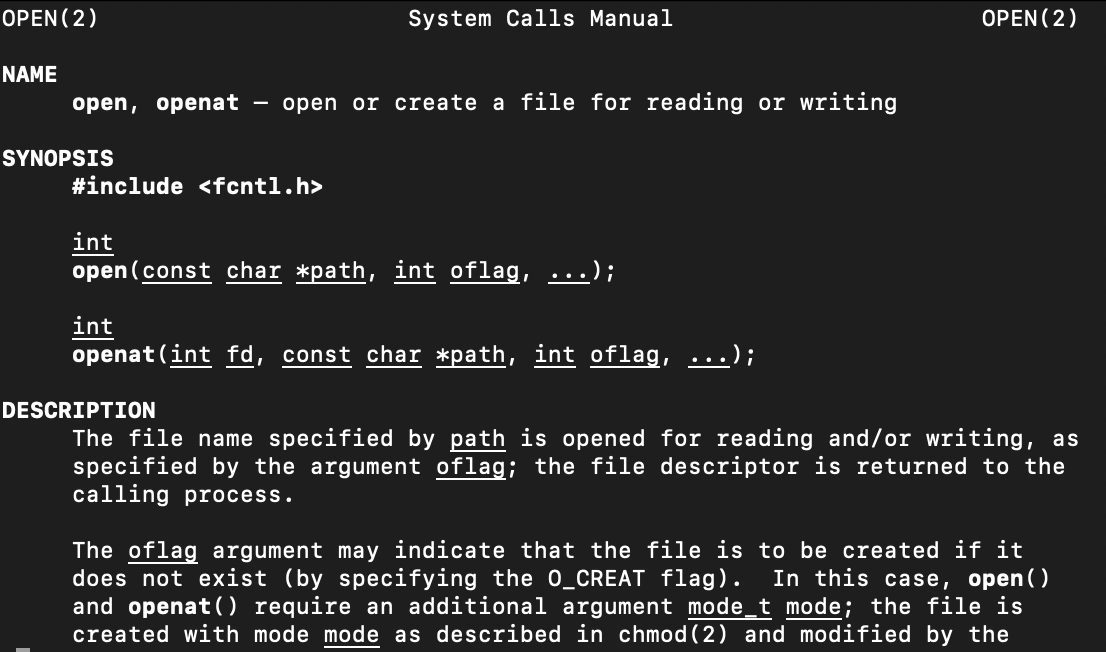
\includegraphics[width=0.8\textwidth]{figures/09-03-open系统调用manu信息.png}
  \caption{open系统调用相关信息}
  \label{fig:open_syscall}
\end{figure}
每个man指令的手册页面都有类似的结构,由以下部分组成
\begin{itemize}
    \item NAME:命令的名称和简短描述
    \item SYNOPSIS:命令的语法和选项 初步描述了命令的基本用法
    \item DESCRIPTION:命令的详细描述和用法
    \item OPTIONS:命令的选项和参数
    \item EXAMPLES:使用命令的示例
    \item FILES:命令可能使用的文件
    \item SEE ALSO:相关命令和手册页面
    \item BUGS:已知的命令错误和限制
    \item AUTHOR:命令的作者和贡献者
\end{itemize}
man是系统的分页(page)手册,指定的man的页选项通常是程序工具或函数名,程序将显示每一项找得到的相关手册页。
如果指定了章节(section),man将在指定章节中搜索。
默认将按照预定的顺序查找所有可用的章节,并且只显示第一个页,即使在多个章节中都存在这个页。
可以在\ref{fig:open_syscall}看到,在man页面的左上角,有一个MAN(2),这里的2就是章节,比较常用的章节号是1、5、8,分别代表用户命令、配置文件和格式、系统管理命令。

通过在文档中找到我们想要的规范信息,我们可以知道实现系统调用的细节规范,如报错类型,返回类型,接口参数等。

接下来,我们以open系统调用为例,来看看如何实现系统调用。
第一步,需要从linux man page中找到open系统调用的系统调用号和函数签名,并将其如\ref{fig:open_syscall1}所示:
\begin{figure}[H]
  \centering
  \includegraphics[width=0.8\textwidth]{figures/09-03-open系统调用函数签名.png}
  \caption{open系统调用号和函数签名}
  \label{fig:open_syscall1}
\end{figure}

第二步,分析该系统调用设计的模块,具体而言是需要实现的功能与内核的哪一个部分关联,例如内存映射、进程管理、进程通信、线程相关等。
之后,分析具体实现的框架,也就是做那些操作,我们需要的函数接口是哪些,从而可以得出一个实现的伪代码。
在open的例子中,我们可以得到如下的伪代码:
\begin{lstlisting}[language=c]
    int open(const char *pathname, int flags, mode_t mode)
    {
        // 1. 检查参数是否合法
        // 2. 从文件系统中找到文件
        // 3. 根据flags和mode参数,检查文件是否可以打开
        // 4. 为文件分配一个文件描述符
        // 5. 返回文件描述符
    }
\end{lstlisting}

最后,在代码实现上,关注手册中的细节,例如可能出现的错误信息,对于特殊情况的处理。
如在open的例子中,可能出现的错误类型有:
\begin{itemize}
    \item EACCES:文件不可访问
    \item EEXIST:文件已经存在
    \item EFAULT:pathname指向的内存空间不可访问
    \item EINTR:调用被信号中断
    \item EISDIR:pathname指向的是一个目录
    \item ELOOP:pathname指向的是一个循环链接
    \item EMFILE:进程打开的文件数超过了系统限制
    \item ENAMETOOLONG:pathname太长
    \item ENFILE:系统打开的文件数超过了系统限制
    \item ENODEV:pathname指向的文件不存在
    \item ENOENT:pathname指向的文件不存在
    \item ENOMEM:内存不足
    \item ENOTDIR:pathname指向的不是一个目录
    \item ENXIO:pathname指向的设备不存在
    \item EOVERFLOW:文件太大
    \item EPERM:pathname指向的文件不可访问
    \item EROFS:pathname指向的文件是只读的
    \item ETXTBSY:pathname指向的文件正在被使用
    \item EWOULDBLOCK:O\_NONBLOCK被设置,但是文件被阻塞
\end{itemize}

如此,我们就完整的实现了一个系统调用。类似的对于其他的系统调用,我们都可以类似的实现。